\documentclass[border=1cm]{standalone}
\usepackage{tikz}
\usetikzlibrary{calc}

\begin{document}

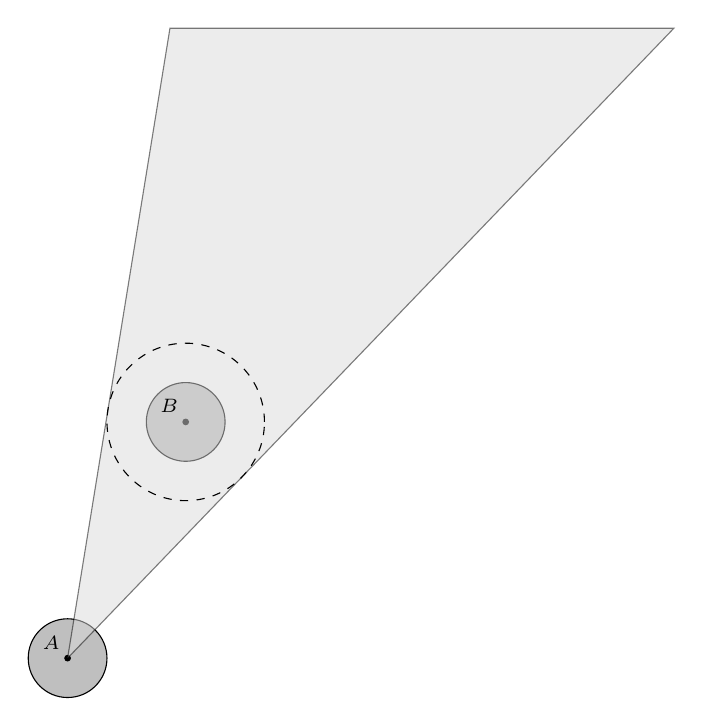
\begin{tikzpicture}
% [trim left=1cm, trim right=1cm, trim top=1cm, trim bottom=1cm]
    % Define points for A and B
    \coordinate (pA) at (0,0);
    \coordinate (pB) at (1.5,3);

    % Draw shaded circles with black outline
    \filldraw[gray!50, draw=black, thin] (pA) circle (0.5cm);
    \filldraw[gray!50, draw=black, thin] (pB) circle (0.5cm);

        % Draw points at the centers of the circles
    \filldraw[black] (pA) circle (1pt);
    \filldraw[black] (pB) circle (1pt);

    % Draw shaded velocity obstacle cone with black outline
    \filldraw[gray!30, draw=black, thin, opacity=0.5] (pA) -- ++(1.3,8) -- ++(6.4,0) -- cycle;


    % Draw dashed circles for Minkowski sum
    \draw[dashed, thin] (pB) circle (1cm);

    % Label points, offset down and to the left
    \node at ($(pA) + (-0.2,0.2)$) {$_A$};
    \node at ($(pB) + (-0.2,0.2)$) {$_B$};

\end{tikzpicture}

\end{document}
